\section{Aritmetica dei calcolatori}

\subsection{Somma e Sottrazione}
Per eseguire l'addizione di due numeri in complemento 
a due dobbiamo eseguire l'addizione bit a bit considerando il riporto.
Mentre per eseguire la sottrazione dobbiamo prima eseguire il complemetno 
a due del secondo membro e poi eseguire la somma.
\paragraph{Overflow}
L'overflow può avvenire quando si esegue la somma di due 
numeri con lo stesso segno oppure quando di esegue la sottrazione di 
numeri con segno opposto.Per identificare l'overflow dobbiamo vedere il 
bit del segno, dato che se i bit del valore non bastano a rappresentare il numero
allora il bit del segno verrà impostato a 1 nel caso di positivi e 0 nel caso di negativi.

\paragraph{Overlflow negli unsigned}
Nei valori unsigned per verificare l'overflow nella somma,
dobbiamo controllare che il risultato sia maggiore dei due
operandi, in caso contrario c'è stato un overflow.
Mentre nella sottrazione dobbiamo verificare che il 
risultato sia minore del minuendo.In caso contrario c'è stato un overflow.

\subsection{Moltiplicazione}

L'hardware per la moltiplicazione è molto simile al modo in cui si esegue la moltiplicazione su carta.

\begin{figure}[H]
    \centering
    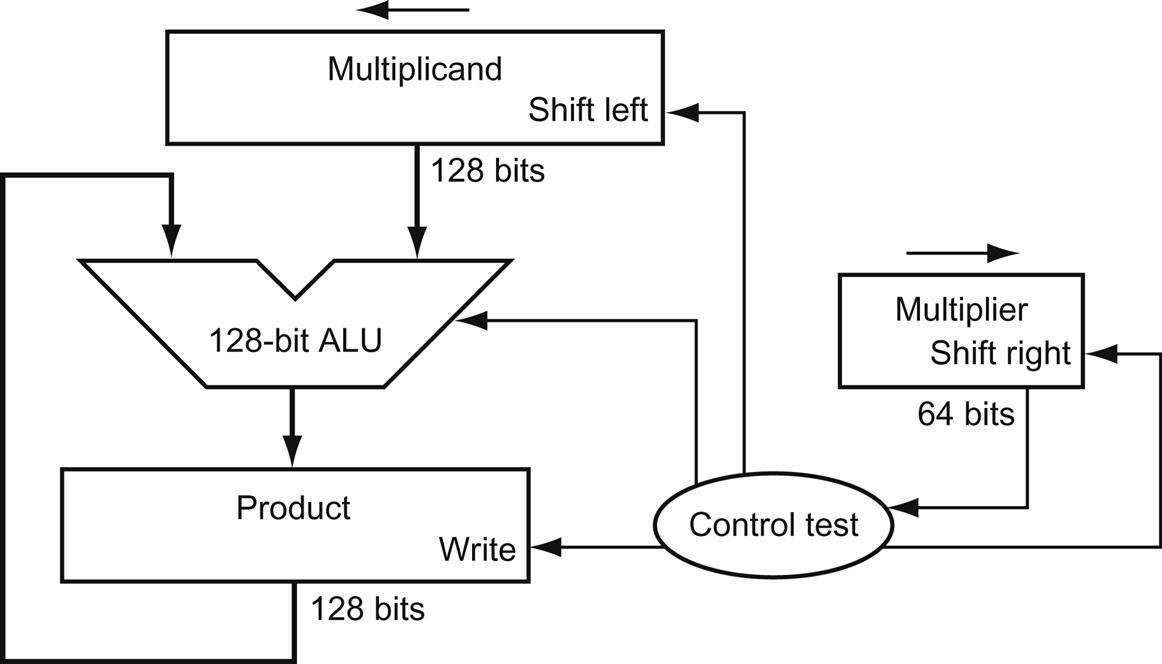
\includegraphics[width=100mm,scale=1.5]{pictures/schemaMoltiplicazione.png}
    \caption{HW moltiplicazione}
    \label{fig:hw-multiplication}
\end{figure}
\newpage
Il control test esegue per 64 volte il seguente algoritmo:
\begin{enumerate}
    \item Controlla che il bit meno valente del moltiplicatore:
    \begin{enumerate}
        \item Se il bit è a 1, allora somma il moltiplicando al prodotto.
        \item Se il bit è a 0, non fa nulla.
    \end{enumerate}
    \item Esegue lo shift left del moltiplicando e lo shift right del moltiplicatore.
\end{enumerate}


\subsubsection{Moltiplicazione migliorato}
Questo hardware può essere rifinito per essere più veloce ed economico.

\begin{figure}[H]
    \centering
    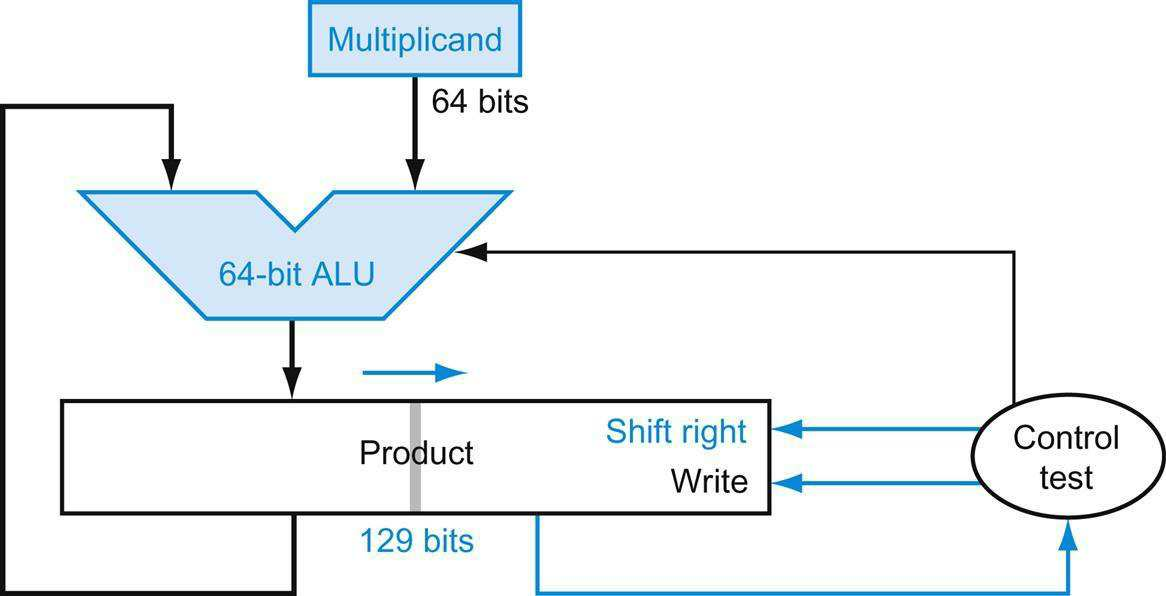
\includegraphics[width=100mm,scale=1.5]{pictures/schemaMoltiplicazioneVeloce.png}
    \caption{HW moltiplicazione migliorato}
    \label{fig:hw-multiplication-improved}
\end{figure}

L'aumento di velocità deriva dall'esecuzione in parallelo, in questo caso lo shift di moltiplicando e moltiplicatore vengono eseguiti 
mentre il moltiplicando viene sommato al prodotto. L'HW deve assicurarsi di testare il giusto bit del moltiplicatore e di 
prendere la versione shiftata del moltiplicando. È più economico perchè non ci serve più una ALU a 128 bits e risparmiamo un 
registro da 128 bits. 

\subsubsection{Moltiplicazione veloce}

Un modo più veloce per eseguire la moltiplicazione è quello di usare un adder per ogni bit del moltiplicatore, in cui
un input è il moltiplicando in cui viene eseguita una AND con il bit del moltiplicatore e l'altro è il risultato di una 
somma precendente. Un modo più efficente però è quello di organizzare i 64 adder in un albero.

\begin{figure}[H]
    \centering
    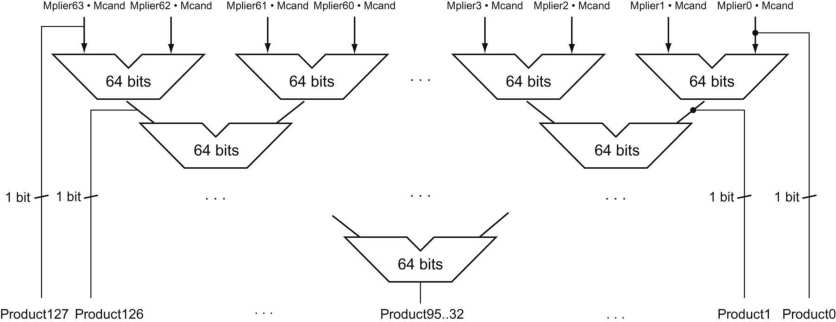
\includegraphics[width=100mm,scale=1.5]{pictures/schema-moltiplicazione-veloce.png}
    \caption{HW moltiplicazione veloce}
    \label{fig:hw-multiplication-fast}
\end{figure}

Questo HW può essere reso più veloce se usiamo dei \textbf{carry save adders} e inoltre è facile implementare una pipeline
per eseguire più moltiplicazioni in parallelo.

\subsection{Divisione}
L'algoritmo per calcolare la divisione, sottrae il divisiore al dividendo, ossia calcola quante volte può essere sottratto 
per calcolare il quoziente.

\begin{figure}[H]
    \centering
    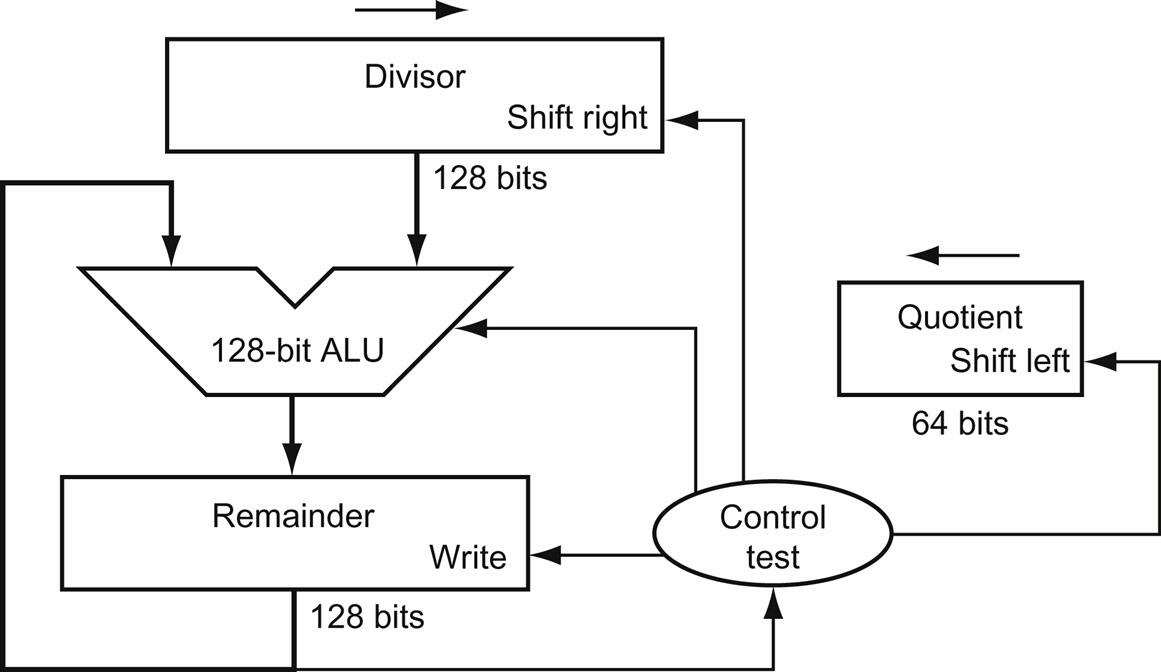
\includegraphics[width=100mm,scale=1.5]{pictures/schema-divisione.png}
    \caption{HW Divisione}
    \label{fig:hw-division}
\end{figure}

Iniziamo con il registro del quozinete a 0, il divisore viene scritto nella metà destra dei 128 bits e il resto è
 inizializzato con il dividendo.

L'HW esegue per 65 volte il seguente algoritmo:
\begin{enumerate}
    \item Si sottrae il divisore al resto.
    \item Si controlla che il resto:
    \begin{enumerate}
        \item Se il resto è positivo si esegue lo shift left con 1 al quoziente.
        \item Se il resto è negativo si esegue lo shift left con 0 al quoziente e si somma il divisore al resto. 
    \end{enumerate}
    \item Si esegue lo shift right del divisore.
\end{enumerate}

\subsubsection{Divisione migliorato}
Si può migliorare l'HW per essere più veloce ed economico. La velocità deriva dell'esecuizione simultante dello 
shifing di Divisore e Quoziente insieme alla sottrazione.
Inoltre usiamo solamente un adder a 64 bit e un solo registro da 129 bits.

\begin{figure}[H]
    \centering
    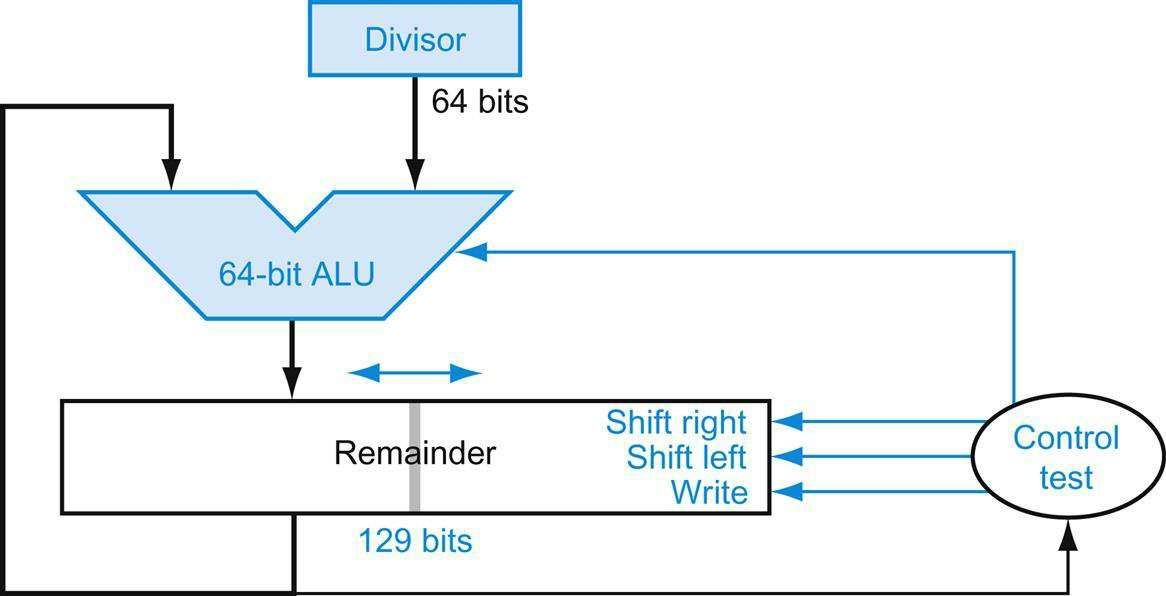
\includegraphics[width=100mm,scale=1.5]{pictures/schema-divisione-bello.png}
    \caption{HW Divisione Migliorato}
    \label{fig:hw-division-improved}
\end{figure}

\subsubsection{Divisione con segno}
Per eseguire la divisione con segno dobbiamo eseguire la divisione normale dei numeri positivi e negare il quoziente 
se i segni di dividendo e divisore non coincidono.

\subsection{Virgola mobile}
I numeri in virgola mobile che rappresentiamo sono tutti in forma normalizzata, ossia con 
una solo cifra dopo la virgola diversa da 0.
Dato che li rappresentiamo in binario sono tutti i numeri della forma $1,xxx..x \times 2^{yy..yy}$.
Quando facciamo un operazione con questi numeri possiamo incorrere in \textbf{overflow} e \textbf{underflow}, il primo si 
ha quando il numero da rappresentare è troppo grande e perciò non ci bastano i bit dell'esponente, mentre il secondo si ha quando il 
numero è troppo piccolo e comunque non ci bastano i bit dell'esponente.

\subsubsection{Eccezioni e Interrupt}
Nel casi \textbf{over/underflow} alcuni computer sollevano un eccezione. Ossia una chiamata a funzione non programmata, in cui 
viene salvato l'indirizzo del codice che ha generato l'eccezione in modo da poter continare la normale esecuzione nel caso 
in cui del codice "risolutivo" venga fornito. 
Nel caso di risc-V non viene sollevata nessuna eccezione, ma per sapere se un over/underflow è avvenuto bisogna leggere 
il registro \textbf{FCSR (Floating-point Control and Status Register)}.

\subsubsection{Somma in virgola mobile}
Per eseguire la somma di due numeri in virgola mobile dobbiamo seguire il seguente algoritmo:
\begin{enumerate}
    \item Si confrontano gli esponenti e si esegue lo shift a destra della mantissa del numero più piccolo affinchè il loro 
    esponente non sia uguale.
    \item Si esegue la somma delle due mantisse
    \item Si normalizza la somma eseguendo degli shift a destra e incrementando l'esponente oppure degli shift a sinistra 
    decrementando l'esponente.
    \item Si controlla la presenza di overflow o underflow e in caso di solleva un eccezione.
    \item Si arrotonda la frazione al numero di bit corretto.
    \item Si controlla se il numero sia sempre normalizzato:
    \begin{enumerate}
        \item Se il numero è normalizzato abbiamo finito.
        \item Se non è normalizzato dobbiamo tornare al passaggio 3.
    \end{enumerate}
\end{enumerate}

\begin{figure}[H]
    \centering
    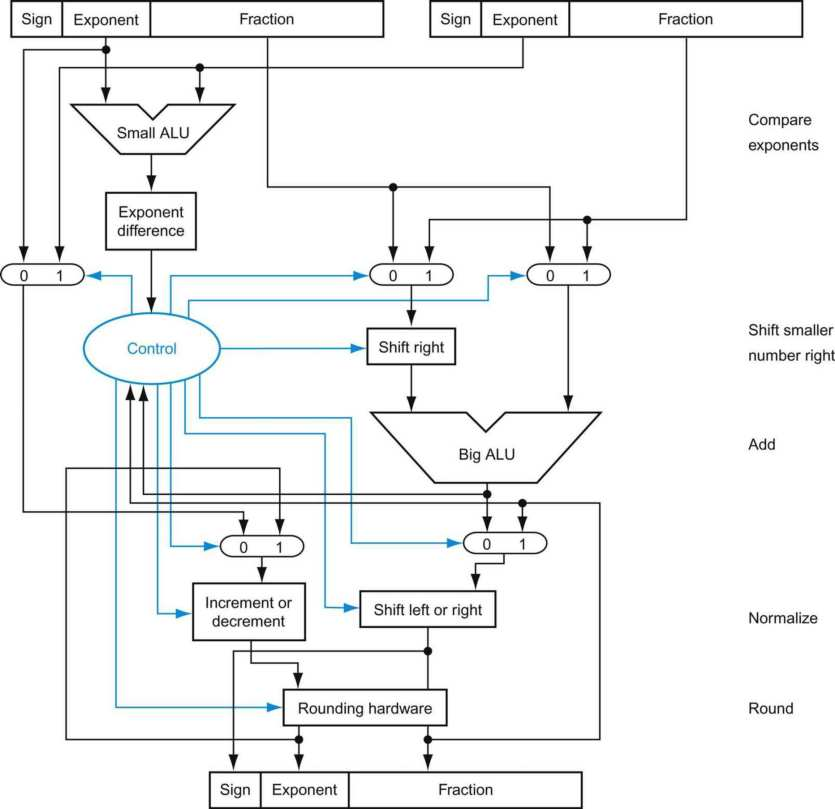
\includegraphics[width=100mm,scale=1.5]{pictures/schema-somma-virgola-mobile.png}
    \caption{HW Somma virgola mobile}
    \label{fig:hw-floating-point-addition}
\end{figure}

